%%%%%%%%%%%%%%%%%%%%%%%%%%%%%%%%%%%%%%%%%%%%%%%%%%%%%%%%%%%%%%%%%%%%%%%%%%%%%%%%%%%%%%%%µ%%%%%%%%%%%
%%%  What's up LOD Cloud - Observing The State of Linked Open Data Cloud Metadata  %%%%
%%%%%%%%%%%%%%%%%%%%%%%%%%%%%%%%%%%%%%%%%%%%%%%%%%%%%%%%%%%%%%%%%%%%%%%%%%%%%%%%%%%%%%%%%%%%%%%%%%%%

\documentclass[runningheads,a4paper]{llncs}

\usepackage[utf8]{inputenc}
\usepackage{amssymb}
\setcounter{tocdepth}{3}
\usepackage{graphicx}
\usepackage{tabularx}
\usepackage{url}
\usepackage{listings}
\usepackage{subfigure}
\usepackage{algorithmic}
\usepackage{algorithm}
\usepackage{xcolor}
\usepackage{caption}
\usepackage{multirow}


\graphicspath{ {figures/} }

\newcommand{\keywords}[1]{\par\addvspace\baselineskip
\noindent\keywordname\enspace\ignorespaces#1}

% todo macro
\usepackage{color}
\newtheorem{deflda}{Axiom}
\newcommand{\todo}[1]{\noindent\textcolor{red}{{\bf \{TODO}: #1{\bf \}}}}

\colorlet{punct}{red!60!black}
\definecolor{background}{HTML}{FFFFFF}
\definecolor{delim}{RGB}{20,105,176}

% Language Definitions for JSON
\lstdefinelanguage{json}{
		basicstyle=\tiny,
    numbersep=4pt,
    showstringspaces=false,
    breaklines=true,
    frame=lines,
    literate=
      {:}{{{\color{punct}{:}}}}{1}
      {,}{{{\color{punct}{,}}}}{1}
      {[}{{{\color{delim}{[}}}}{1}
      {]}{{{\color{delim}{]}}}}{1},
}

%%%%%%%%%%%%%%%%%%%%%%%%%%%%%%%
%%%  Beginning of document  %%%
%%%%%%%%%%%%%%%%%%%%%%%%%%%%%%%

\begin{document}

% first the title is needed
\title{What's up LOD Cloud}
\subtitle{Observing The State of Linked Open Data Cloud Metadata}

\author{Ahmad Assaf\inst{1}\inst{2}, Aline Senart\inst{2} and Rapha\"{e}l Troncy\inst{1} }

\institute{EURECOM, Sophia Antipolis, France. \email{<firstName.lastName@eurecom.fr>}
  \and SAP Labs France. \email{<firstName.lastName@sap.com>}
}

% a short form should be given in case it is too long for the running head
\titlerunning{Observing The State of Linked Open Data Cloud Metadata}
%\authorrunning{Assaf, Senart and Troncy}

\maketitle

%%%%%%%%%%%%%%%%%%
%%%  Abstract  %%%
%%%%%%%%%%%%%%%%%%

\begin{abstract}
Linked Open Data (LOD) has emerged as one of the largest collections of interlinked datasets on the web. In order to benefit from this mine of data, one needs to access to descriptive information about each dataset (or metadata). This information can be used to delay data entropy, enhance datasets discovery, exploration and reuse as well as helping data portal administrators in detecting and eliminating spam. However, such metadata information is currently very limited to a few data portals where they are usually provided manually, thus being often incomplete and inconsistent in terms of quality. To address these issues, we propose a scalable automatic approach for extracting, validating, correcting and generating descriptive linked dataset profiles. This approach applies several techniques in order to check the validity of the metadata provided and to generate descriptive and statistical information for a particular dataset or for an entire data portal.

% We target CKAN powered data portals and validate our framework on the Linked Open Data (LOD) cloud. The results demonstrate that the general state of LOD cloud needs more attention as most of the datasets suffer from bad quality metadata lacking some informative metrics needed to facilitate dataset search. The noisiest metadata values were access information such as licensing information, resource descriptions as well as resource reachability problems.

\keywords{Linked Data, Dataset Profile, Metadata, Data Quality}
\end{abstract}

%%%%%%%%%%%%%%%%%%%%%%%%%
%%%  1. Introduction  %%%
%%%%%%%%%%%%%%%%%%%%%%%%%

\section{Introduction}
\label{sec:introduction}

\section{Related Work}
\label{sec:related-work}



%%%%%%%%%%%%%%%%%%%%%%%%%%%%%%%%%%%%%%%
%%%  2. Experiments and Evaluation  %%%
%%%%%%%%%%%%%%%%%%%%%%%%%%%%%%%%%%%%%%%

\section{Experiments and Evaluation}
\label{sec:experiment}

In this section, we provide the experiments and evaluation of the proposed framework. All the experiments are reproducible by our tool and their results are available on the its Github repository.\\
We have run the framework on the LOD cloud containing 259 datasets at the time of writing this paper. We ran the instance and resource extractor in order to cache the metadata files for these datasets locally and ran the validation process which took around one and a half hour on a 2.6 Ghz Intel Core i7 processor with 16GB of DDR3 memory machine.\\
A CKAN dataset metadata describes three main sections in addition to the core dataset's properties. Those are the groups, tags and resources. Each section contains a set of metadata corresponding to one or more metadata type. For example, a dataset resource will have general information such as the resource name, access information such as the resource url and provenance information such as creation date. The framework generates a report aggregating all the problems in all these sections, fixing field values when possible. Errors can be the result of missing metadata fields, undefined field values or field value errors e.g., unreachable URL or incorrect email address.

Figures \ref{fig:2} and \ref{fig:3} show the percentage of errors found in metadata fields by section and by information type respectively. We found out that the most erroneous information for the dataset core information were ownership related as 41\% were missing or undefined. Datasets resources have the poorest metadata. 64\% of the general metadata, all the access information and 80\% of the provenance information contained missing or undefined values. Table \ref{tab:main} shows the top metadata fields errors in each metadata information type.

\begin{center}
\begin{tabular}{|c|c|c|c|c|c|}

\hline
\multicolumn{2}{|c|}{Metadata Field} & Error \% & Section & Error Type & Auto Fix\tabularnewline
\hline
\hline
\multirow{6}{*}{General } & group & 100\% & Dataset & Missing & -\tabularnewline
\cline{2-6}
 & vocabulary\_id & 100\% & Tag & Undefined & -\tabularnewline
\cline{2-6}
 & url-type & 96.82\% & Resource & Missing & -\tabularnewline
\cline{2-6}
 & mimetype\_inner & 95.88\% & Resource & Undefined & Yes\tabularnewline
\cline{2-6}
 & hash & 95.51\% & Resource & Undefined & Yes\tabularnewline
\cline{2-6}
 & size & 81.55\% & Resource & Undefined & Yes\tabularnewline
\hline
\multirow{5}{*}{Access } & cahce\_url & 96.9\% & Resource & Undefined & -\tabularnewline
\cline{2-6}
 & webstore\_url & 91.29\% & Resource & Undefined & -\tabularnewline
\cline{2-6}
 & license\_url & 54.44\% & Dataset & Missing & Yes\tabularnewline
\cline{2-6}
 & url & 30.89\% & Resource & Unreachable & -\tabularnewline
\cline{2-6}
 & license\_title & 16.6\% & Dataset & Undefined & Yes\tabularnewline
\hline
\multirow{5}{*}{Provenance } & cache\_last\_updated & 96.91\% & Resource & Undefined & Yes\tabularnewline
\cline{2-6}
 & webstore\_last\_updated & 95.88\% & Resource & Undefined & Yes\tabularnewline
\cline{2-6}
 & created & 86.8\% & Resource & Missing & Yes\tabularnewline
\cline{2-6}
 & last\_modified & 79.87\% & Resource & Undefined & Yes\tabularnewline
\cline{2-6}
 & version & 60.23\% & Dataset & Undefined & -\tabularnewline
\hline
\multirow{5}{*}{Ownership } & maintainer\_email & 55.21\% & Dataset & Undefined & -\tabularnewline
\cline{2-6}
 & maintainer & 51.35\% & Dataset & Undefined & -\tabularnewline
\cline{2-6}
 & author\_email & 15.06\% & Dataset & Undefined & -\tabularnewline
\cline{2-6}
 & organization\_image\_url & 10.81\% & Dataset & Undefined & -\tabularnewline
\cline{2-6}
 & author & 2.32\% & Dataset & Undefined & -\tabularnewline
\hline
\end{tabular}
\captionof{table}{Top metadata fields error \% by type} \label{tab:main}
\end{center}

\begin{figure}

\parbox{7cm}{\hspace*{-.2in}
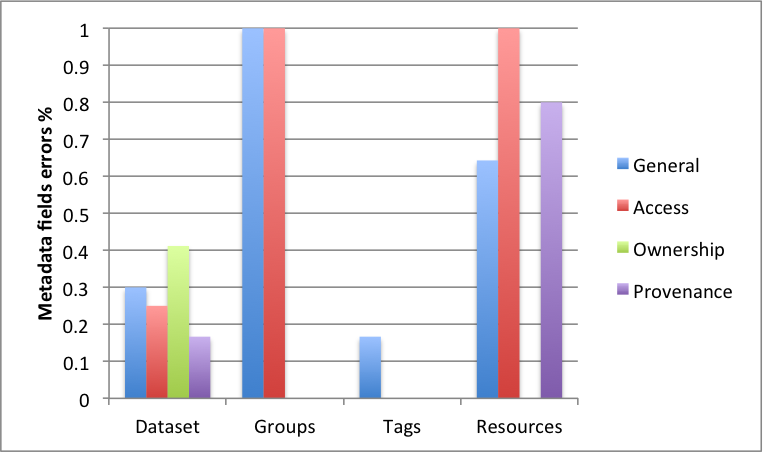
\includegraphics[width=.95\linewidth]{metadata_noise_by_section.png}
\captionsetup{textfont=small,singlelinecheck=off,justification=centering}
\caption{Error \% by section}
\label{fig:2}}
\qquad
\begin{minipage}{7cm}\hspace*{-.6in}
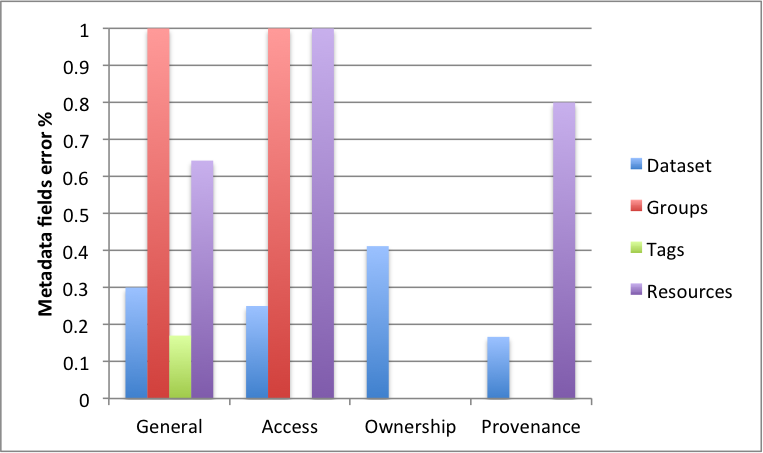
\includegraphics[width=.95\linewidth]{metadata_noise_by_metadata_type.png}
\captionsetup{textfont=small,singlelinecheck=off,justification=raggedright}
\caption{Error \% by information type}
\label{fig:3}
\end{minipage}

\end{figure}

We notice that 42.85\% of the top metadata problems can be fixed automatically. 44.44\% of these problems can be fixed by our tool while the others need tools that are plugged into the data portal. We further present and discuss the results grouped by metadata information type below.

\subsection{General information} 34 datasets (13.13\%) did not have valid \texttt{notes} values. \texttt{tags} information for the datasets were complete except for the \texttt{vocabulary\_id} as it was missing from all the datasets' metadata. All the datasets \texttt{groups} information were missing \texttt{display\_name, description, title, image\_display\_url, id, name}. After \\manual examination, we noticed a clear overlap between group and organization information. Many datasets like \texttt{event-media} used the organization field to show group related information (being in LOD Cloud) instead of the publishers details.\\

\subsection{Access information} 25\% of the datasets access information (being the dataset URL and any URL defined in its groups) has issues related to them (missing or unreachable URLs).
Three datasets (1.15\%) did not have a URL defined (tip, uniprot\-databases, uniprot\-citations) while 45 datasets (17.3\%) defined URLs were not accessible at the time writing this paper. One dataset did not have resources information (bio2rdf\-chebi) while the other datasets had a total of 1068 defined resources.\\
On the datasets resources level, we noticed wrong or inconsistent values in the \texttt{size} and \texttt{mimetype} fields. 20 (1.87\%) resources had incorrect \texttt{mimetype} defined, while 52 (4.82\%) had incorrect \texttt{size} values. These values have been automatically fixed based on the values defined in the HTTP response header. However, 44 datasets have valid \texttt{size} field values and 54 have valid \texttt{mimetype} field values where they were not reachable, thus providing incorrect information.\\
15 (68\%) fields of all the other access metadata are missing or have undefined values. Looking closely, we noticed that most of these problems can be easily fixed automatically by tools that can be plugged to the data portal. For example, the top six missing fields are the \texttt{cache\_last\_updated}, \texttt{cache\_url}, \texttt{url\-type}, \texttt{webstore\_last\_updated}, \texttt{mimetype\-\_inner} and \texttt{hash} which can be computed and filled automatically. However, the most important missing information which require manual entry are the dataset's \texttt{name} and \texttt{description} were missing from 817 (76.49\%) and 98 (9.17\%) resources respectively.
A total of 334 resources (31.27\%) URLs were not reachable, thus affecting highly the availability of these datasets. CKAN resources can be of various predefined types $(file, file.upload, api, visualization, code and documentation)$. The frameowork also breaks down these unreachable resources according to their types. 211 (63.17\%) resources did not have valid \texttt{resource\_type}, 112 (33.53\%) were files, 8 (2.39\%) and one (0.029\%) metadata, example and documentation types.

To have more details about the resources URL types, we created a $key:object meta-field values$ group level report on LOD cloud with \texttt{resources>\\format:title}. This will aggregate the resources format information for each dataset. We found out that only 161 (62.16\%) of the datasets valid URLs have SPARQL endpoints defined by \texttt{api/sparql} resource format. 92.27\% provided RDF example links and 56.3\% provided direct links to RDF down-loadable dumps.

The noisiest part of the access metadata was license information. A total of 43 datasets (16.6\%) did not have a defined \texttt{license\_title} and \texttt{license\_id} fields, where 141 (54.44\%) had missing \texttt{license\_url} field. However, we managed to normalize 123 (47.49\%) of the datasets' license information using the manual mapping file.

\subsection{Ownership information} Ownership information is divided into direct ownership (author and maintainer) and organization information. Four fields (66.66\%) of the direct ownership information were missing or undefined. The breakdown for the missing information is: 55.21\% \texttt{maintainer\_email}, 51.35\% \texttt{maintainer}, 15.06\% \texttt{author\_email}, 2.32\% \texttt{author}. Moreover, our framework performs checks to validate existing email values. 11 (0.05\%) and 6 (0.05\%) of the defined \texttt{author\_email} and \texttt{maintainer\_email} fields were not valid email addresses respectively.\\
For the organization information, two field values (16.6\%) were missing or undefined. 1.16\% of the \texttt{organization\_description} and 10.81\% of the \texttt{organization\-\_image\_url} information with two out of these URLs were unreachable.

\subsection{Provenance information} 80\% of the resources provenance information were missing or undefined. However, most of the provenance information e.g., \texttt{metadata\_created, \\metadata\_modified)} can be computed automatically by tools plugged into the data portal. The only field requiring manual entry is the \texttt{version} field which was found to be missing from 60.23\% of the datasets.

%%%%%%%%%%%%%%%%%%%%%%%%%%%%%%%%%%%%%%%
%%%  5. Conclusion and Future Work  %%%
%%%%%%%%%%%%%%%%%%%%%%%%%%%%%%%%%%%%%%%
\section{Conclusion and Future Work}
\label{sec:conclusion}

In this paper, we proposed a scalable automatic approach for extracting, validating, correcting and generating descriptive linked dataset profiles. This approach applies several techniques in order to check the validity of the metadata provided and to generate descriptive and statistical information for a particular dataset or for an entire data portal. Based on our experiments running the tool on the LOD cloud, we discovered that the general state of the datasets needs attention as most of them lack informative access information and their resources suffer low availability. These two metrics are of high importance for enterprises looking to integrate and use external linked data.

It has been noticed that the issues surrounding metadata quality affect directly dataset search as data portals rely on such information to power their search index. We noted the need for tools that are able to identify various issues in this metadata and correct them automatically. We found out that 32.25\% of all the metadata information can be automatically fixed, on which 50\%of them can be directly fixed by our framework. The rest are mainly provenance information that requires special treatment.

As part of our future work, we plan to introduce workflows that will be able to correct the rest of the metadata either automatically or through intuitive manually-driven interfaces. We also plan to integrate statistical and topical profilers to be able to generate full comprehensive profiles. We also intend to suggest a ranked standard metadata model that will help generate more accurate and scored metadata quality profiles. We also plan to run this tool on various CKAN based data portals, schedule periodic reports to monitor the evolvement of datasets metadata. Finally, at some stage, we plan to extend this tool for other data portal types like DKAN and Socrata.


\bibliographystyle{abbrv}
\nocite{*}
\bibliography{SOLD}
\end{document}
